%# -*- coding: utf-8-unix -*-
%%==================================================
%% chapter02.tex for SJTU Master Thesis
%%==================================================

\chapter{Shuffle的优化策略}
\label{optimization}

本章将详细阐述实现shuffle优化的方法论。
首先SCache通过提供shuffle读写API的方式来实现shuffle在计算任务中的解耦。
其次SCache通过对shuffle结合应用上下文的外部管理,实现了一个跨平台的通用优化方案。
然后SCache通过两个启发式算法来实现对于shuffle依赖的预调度和数据预取,来实现shuffle传输时间的优化。
最后,SCache通过结合应用上下文的内存管理,来给shuffle数据提供高效的内存缓存,加速读写。

\section{Shuffle的解耦合}

要将shuffle从DAG计算任务中解耦,需要同时解决map任务与reduce任务的紧耦合。

在map任务完成计算之后,会产生一个键值对的集合,表示该任务计算的输出结果。
之后map任务则会根据用户定义的分区函数(比如哈希,排序等)来对这些键值对进行分块存储。
其中每一个数据块存储的是下一个reduce阶段其中一个任务的部分输入数据。
在进行分块的过程中,这些键值对就会被map任务写入到磁盘相应的文件中。
以上过程就是shuffle在map阶段的磁盘写操作,也就是图\ref{fig:workflow}中的“shuffle write”部分。
结合图\ref{fig:util}可以发现,在进行这部分操作时,并不需要大量的CPU资源。
而且由于计算已经完成,分配给该任务的slot中计算资源部分也应当在此处被释放。
因此为了实现更细粒度的硬件资源管理,必须将这部分I/O操作从计算任务中解耦出来。
为了实现该部分的解耦,SCache采用了内存拷贝的技术。
即通过修改DAG计算框架的部分代码,使得map任务在进行键值对分区时通过内存拷贝,将分区好的键值对数据块移动到SCache的内存空间。
而在内存拷贝完成之后,该任务的slot就会被立即释放。

在reduce阶段,每一个任务开始之前,都会通过网络从远程节点的磁盘中拉取该任务需要的shffle数据块,也就是图\ref{fig:workflow}中的“shuffle read”部分。
与map任务相似,在执行shuffle数据拉取的过程中,CPU资源将会被闲置。
但是与map任务不同的是,由于shuffle数据的拉取实在任务开始之前,所以要优化这部分开销,就需要提前读取shuffle数据到本地节点,也就是shuffle数据的预取。
为了实现shuffle数据的预取,SCache会根据任务预调度的结果,在map阶段就开始shuffle的数据读取。
于此同时,通过结合DAG计算框架的任务调度信息来对预取的shuffle数据提前进行内存缓存。
与map任务类似,当reduce任务开始执行时,可以通过调用SCache的API来实现以内存拷贝的方式从本地读取shuffle数据。

通过以上方法,SCache将shuffle相关的I/O操作从map任务与reduce任务两端都进行了解耦合,将I/O资源的管理从DAG计算框架原本粗粒度的slot中进行分离,实现了更细粒度的硬件资源分配管理。
而DAG计算框架仅仅需要完成计算任务与计算密集型资源的管理,使得硬件资源利用率得到了很大提升。

\section{结合上下文的任务预调度}

为了优化shuffle在reduce任务段的开销,必须实现对shuffle数据的预取。
而shuffle数据与reduce任务是一一对应关系,当reduce任务被DAG计算框架调度到某个节点之前,shuffle预取的目的节点也是未知的。
因此要实现shuffle数据的预取,首先需要实现对reduce任务的预调度。
在目前的DAG计算框架当中,Hadoop MapReduce通过slow-start\cite{hadoop}的方案来实现了reduce任务在map阶段的预调度。
这种预调度存在的最大问题就是会占用部分计算的资源(slot)。
为了解决这个困境,SCache提出了一种辅助调度的策略。
即在map阶段,SCache通过上下文信息和map任务执行的中间状态对reduce任务进行预调度。
这一轮预调度只会产生一个reduce任务与节点的映射关系,从而是的shuffle数据预取成为可能。
而slot在这一轮预调度中并不会被占用,从而避免影响map阶段的性能。
于此同时,当map阶段执行结束,DAG计算框架开始调度reduce任务时,通过相应接口访问SCache的调度器,从而获取相应的预调度结果。
通过这种协同调度的方式,SCache实现了预调度但是不占用计算资源的任务调度机制,从而解决了由于任务节点映射未知而无法进行shuffle数据预取的困境。

\subsection{随机任务预调度的问题}

实现任务预调度最简单的方式便是随机均匀的将下一阶段的任务分配到各个计算节点上。
虽然这种简单的随机调度能保证各个节点在任务数目上的均衡,但是真正的负载并不仅取决于任务数目,也需要考虑每个任务所需要计算的数据量。
在图\ref{fig:sim}中我们展现了在OpenCloud\footnote{http://ftp.pdl.cmu.edu/pub/datasets/hla/dataset.html}公开的任务运行日志对不同任务预调度算法的性能测试。
在这里我们比较了三种不同的调度算法的在调度不同轮次的任务时性能,包括随机调度算法,Spark默认调度算法(FIFO)以及我们提出的基于启发式的最小堆算法。
图\ref{fig:sim}中的红色点状线段为比较基准线,通过计算在Spark默认调度算法下的计算阶段完成时间来获得。
然后我们假设在shuffle数据已经获得预取的情况下,移除了日志中shuffle读取的时间开销,然后比较了以上三个算法对于基准线的性能变化。
需要注意的是在OpenCloud公开的工作日志中,大部分工作都只包含了少量的shuffle开销。
图\ref{fig:cdf}展现了在OpenCloud日志中shuffle传输时间占整个redue计算阶段完成时间的累积分布。
其平均shuffle传输时间只占到了reduce阶段完成时间的3.2\%。

\begin{figure}[!htp]
    \centering
    \begin{minipage}[t]{0.55\textwidth}
	    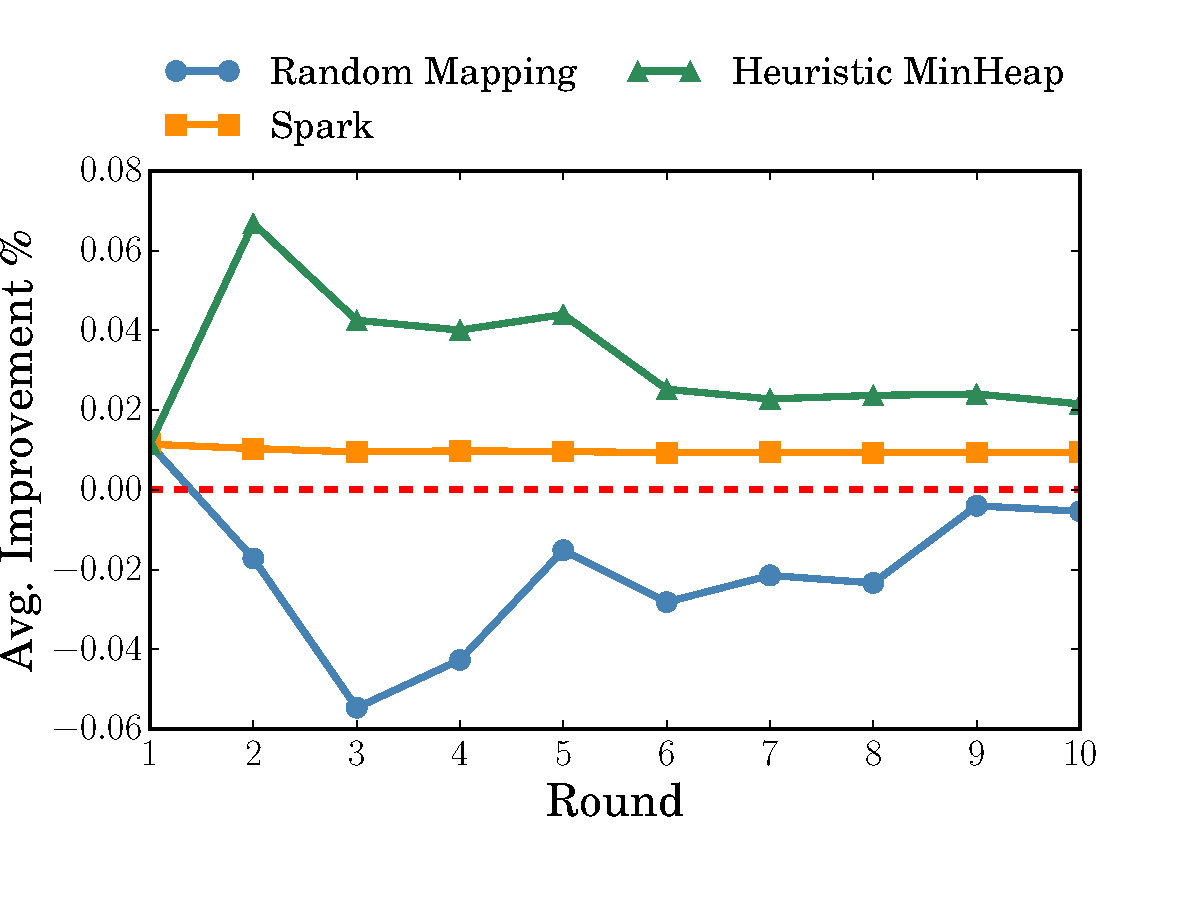
\includegraphics[width=\textwidth]{../../PPoPP-2018/fig/sim.pdf}
	    \bicaption[fig:sim]{基于OpenCloud日志的计算阶段完成时间提升}{基于OpenCloud日志的计算阶段完成时间提升}{Fig}{Stage Completion Time Improvement of OpenCloud Trace}
    \end{minipage}
    \begin{minipage}[t]{0.4\textwidth}
	    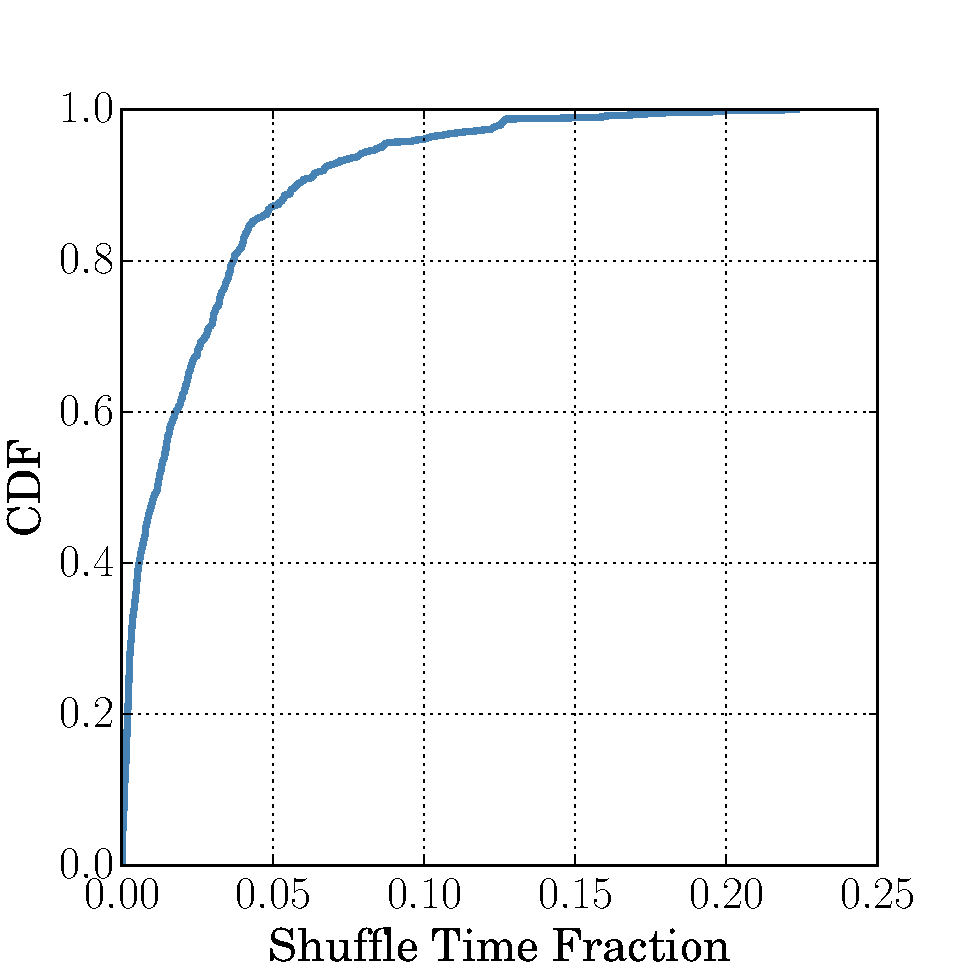
\includegraphics[width=\textwidth]{../../PPoPP-2018/fig/reduce_cdf.pdf}
	    \bicaption[fig:cdf]{OpenCloud日志中shuffle时间占比累积分布}{OpenCloud日志中shuffle时间占比累积分布}{Fig}{Shuffle Time Fraction CDF of OpenCloud Trace}
    \end{minipage}
\end{figure}

虽然这是一个轻量shuffle的工作日志,但是在模拟中我们发现随机调度算法仅仅只能在只有一轮计算任务的情况下获得一个较好的性能提升。
随着任务执行轮次的增加,随机调度算法的性能甚至不如没有经过shuffle预取优化的基准线。
究其原因,是由于在分布式DAG计算过程当中,普遍存在数据分区之后体积的分布不均,存在倾斜(data skew)\cite{reining, gufler2012load, skewtune}。
在随机调度算法中,可能会把几个输入数据相对较大的任务调度到一个节点上。
因为受限于BSP的同步模式,一个计算阶段的完成需要等到该阶段所有任务的完成。
这种缓慢任务的碰撞会拖慢整个计算阶段的完成,进而使得性能甚至不如没有优化的基准线。
更重要的是,随机调度完全忽略了shuffle数据的本地性,因而可能在shuffle网络传输阶段引入额外的流量开销。

\subsection{对shuffle数据分布的预测}

随机任务预调度之所以会造成这些问题是因为在调度过程中完全忽略了应用的上下文信息,比如map阶段产生的shuffle数据的体积分布等。
而一个较优的调度结果可以在该reduce计算阶段总共依赖的shuffle数目,该reduce阶段的任务数目(即shuffle数据块个数)以及每个shuffle中数据块体积这些参数都已知的情况下做出。
在这些都已知的情况下,如果不考虑数据本地性,则该调度问题可以被转化为经典的makespan问题,通过近似算法可以获得至少2倍于最优值的调度结果\cite{approximation}。
而这三个参数中,对于reduce计算阶段的shuffle依赖数目以及该阶段的任务数目都可以通过提取DAG计算框架中的应用信息来获取。
比如Spark在生成RDD的转换关系的同时,就可以获取这两者的信息\cite{spark}。
在此基础上,如果可以对shuffle数据的体积进行相对准确的预测,那么就可以基于此做出一个较优的预调度结果。

\begin{figure}[!htp]
	\centering
	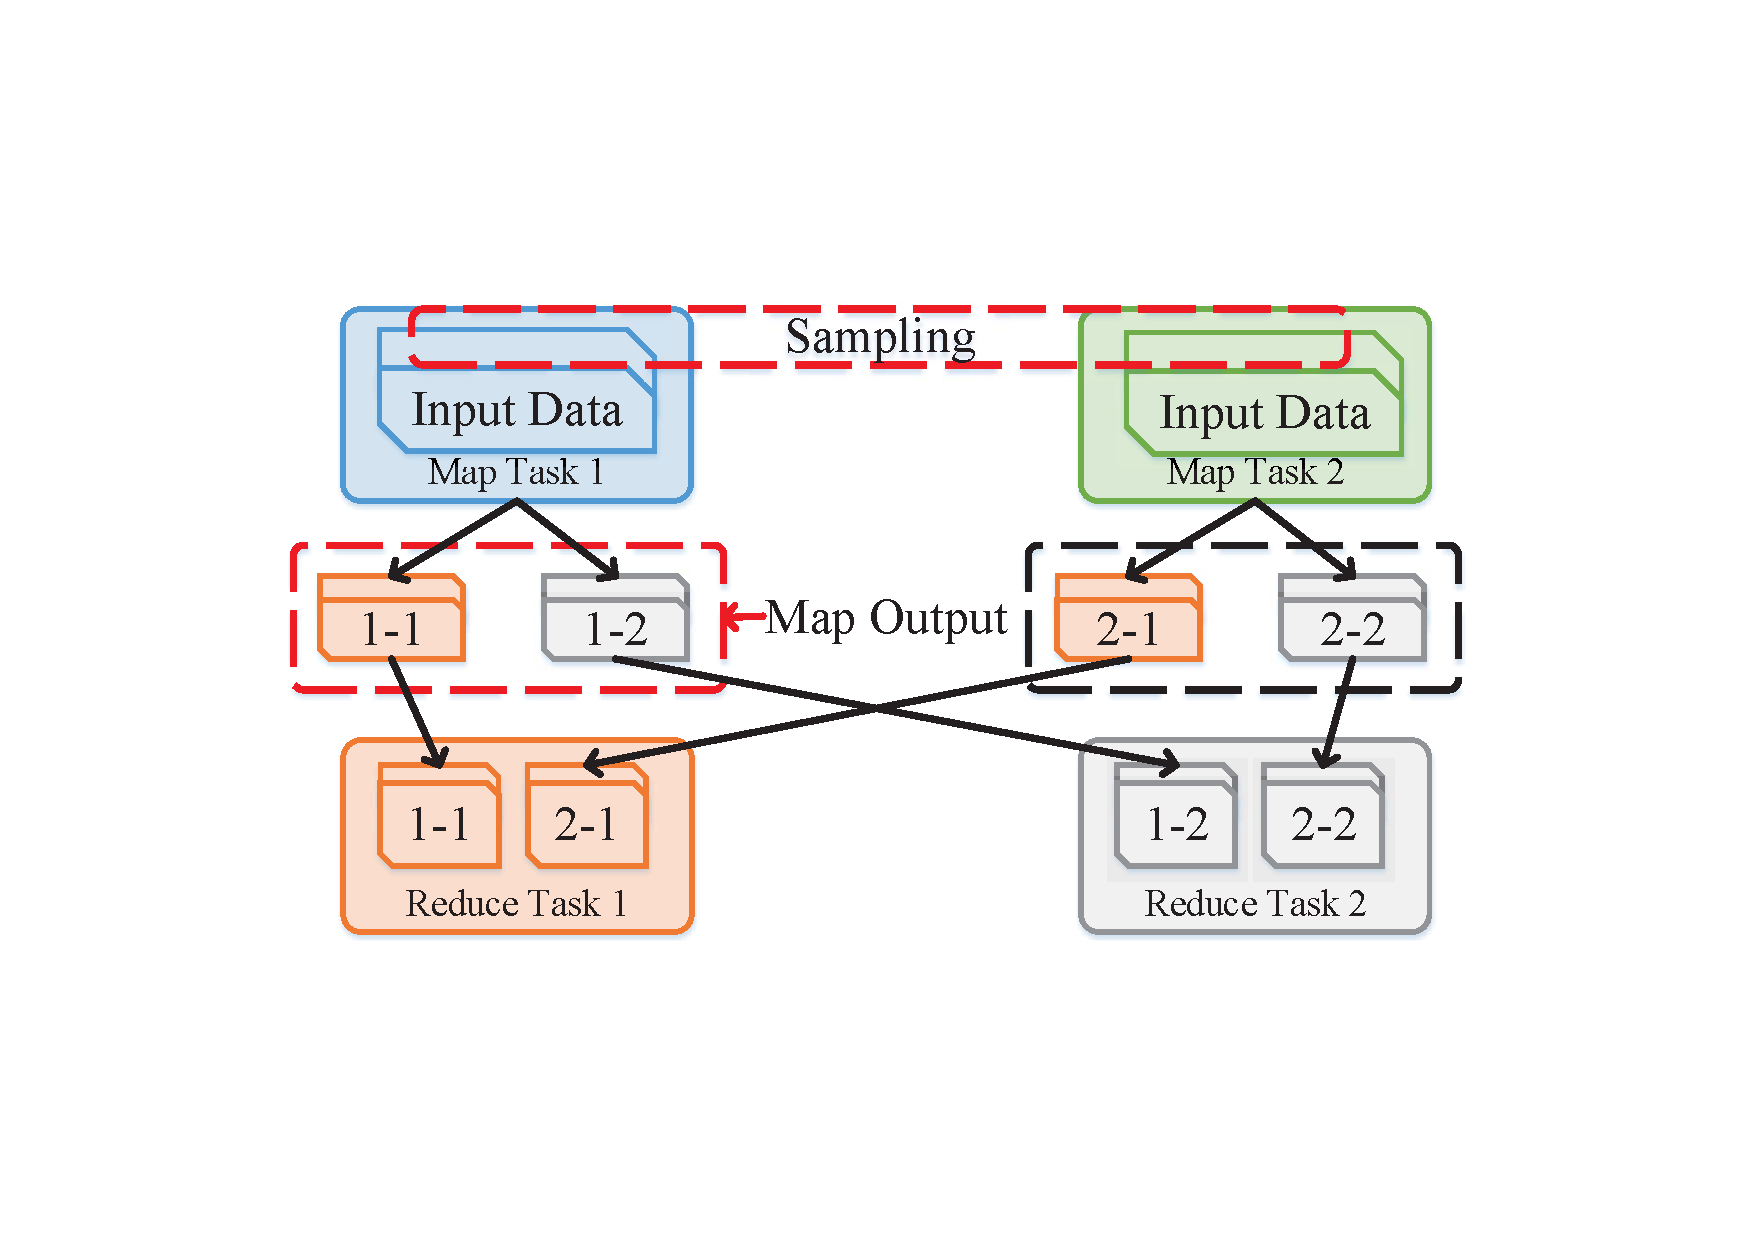
\includegraphics[width=0.6\textwidth]{../../PPoPP-2018/fig/shuffle.pdf}
	\bicaption[fig:shuffle]{Shuffle数据分布预测示意图}{Shuffle数据分布预测示意图}{Fig}{Shuffle Data Prediction}
\end{figure}

如图\ref{fig:shuffle}所示,根据DAG的计算流程,每一个reduce任务需要获取的shuffle数据取决于:上一阶段map任务的输入数据体积,map任务的计算过程和用户定义的分区函数。
对于map阶段的每一个计算任务,都会产生一个对应于reduce阶段某一个任务的数据块。
因此reduce阶段一个任务的输入数据体积大小$reduceSize_i = \sum_{j=0}^{m} {BlockSize_{ji}}$,其中$m$代表map阶段任务的数目。
$BlockSize_{ji}$代表了这个数据块是由第$j$个map任务产生,属于第$i$个reduce任务的输入(比如图\ref{fig:shuffle}中数据块“1-1”)。

对于一些DAG较为简单的应用,比如Hadoop MapReduce的中工作\cite{hadoop},由于reduce阶段的shuffle的依赖往往只有一个,因此对于shuffle数据分布的预测就相对容易。
许多研究工作证明,对于此类工作,在执行工作的配置没有改变的情况下,上文所提到的$BlockSize_{ji}$可以通过简单的线性回归模型获取比较高的预测精度\cite{ishuffle, predict}。
这种线性回归模型采用了对已经运行结束的map任务产生的shuffle数据块进行统计,获取当前这些数据块中属于不同reduce任务的体积,然后采用线性回归的方法,结合剩余map任务的个数以及其相应的输入数据来对最终shuffle的数据分布做出预测。

但是随着DAG框架的演化,计算逻辑的表达和数据依赖关系变得日趋复杂。这些计算过程中的不确定性都会影响到shuffle数据的预测精度。
比如在Spark中一个由用户自定义的数据分区函数就有可能会使当前已经获取的map任务产生的shuffle数据分布与最终的shuffle数据分布产生巨大的不一致性。

为了更直观地展示这种不一致性,我们对不同的数据集输入在不同分区函数情况下应用线性回归模型预测的结果进行了测试。
如图

\begin{figure}[!htp]
    \centering
    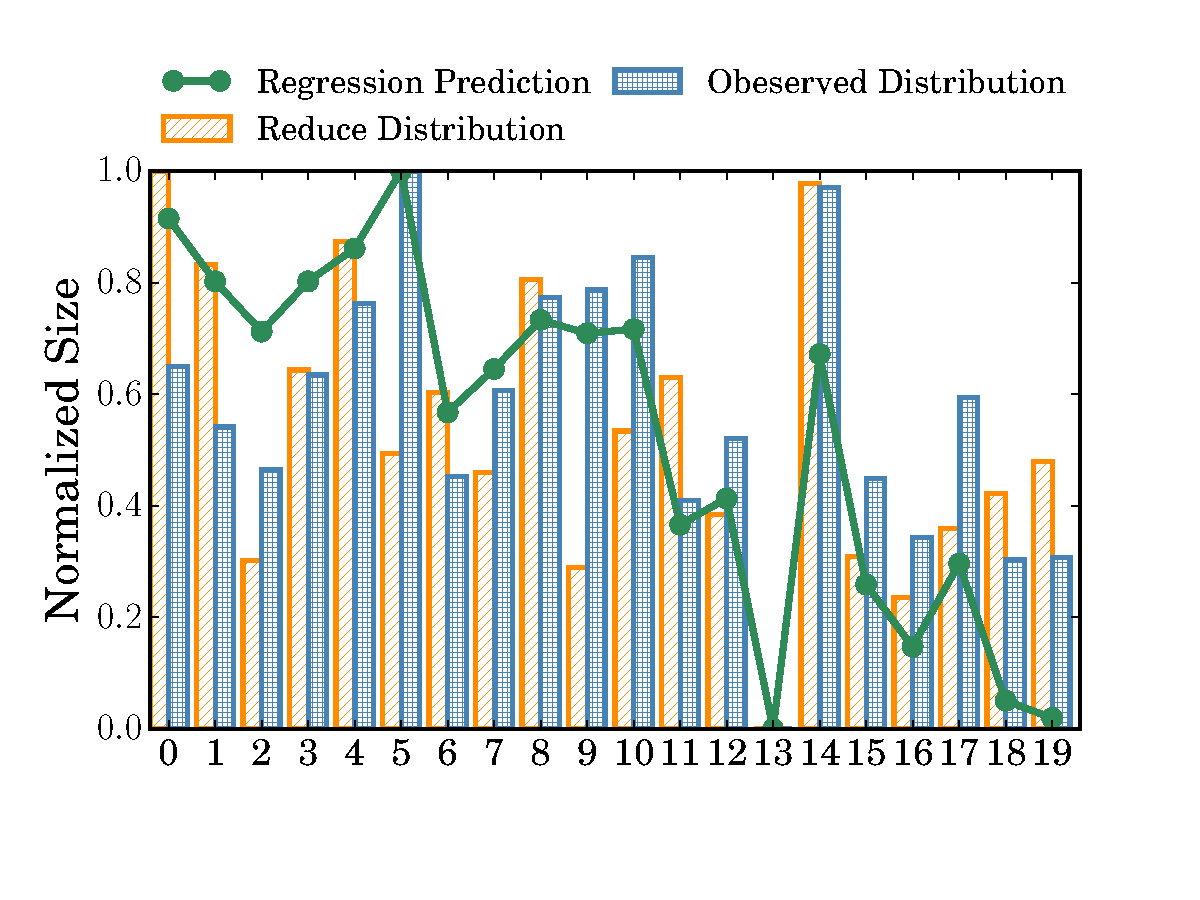
\includegraphics[width=0.6\textwidth]{../../PPoPP-2018/fig/hash_pre.pdf}
	\bicaption[fig:hash_pre]{哈希分区函数下线性回归预测结果}{哈希分区函数下线性回归预测结果}{Fig}{Linear Regression Prediction of Hash Partitioner}
\end{figure}

\begin{figure}[!htp]
    \centering
	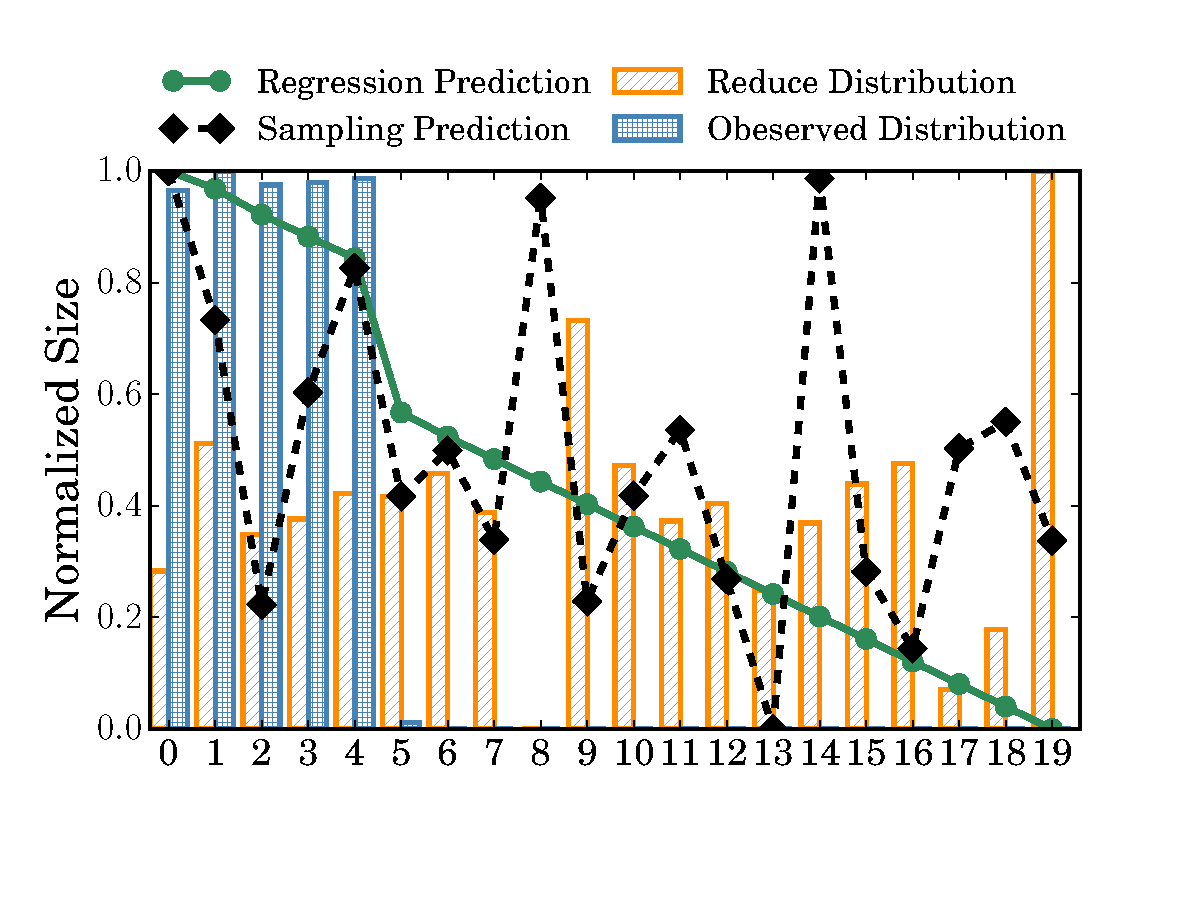
\includegraphics[width=0.6\textwidth]{../../PPoPP-2018/fig/range_pre_sample.pdf}
	\bicaption[fig:range_pre_sample]{范围分区函数下线性回归预测与采样预测的结果}{范围分区函数下线性回归预测与采样预测的结果}{Fig}{Linear Regression and Sampling Prediction of Range Partitioner}
\end{figure}

\begin{figure}[!htp]
    \centering
	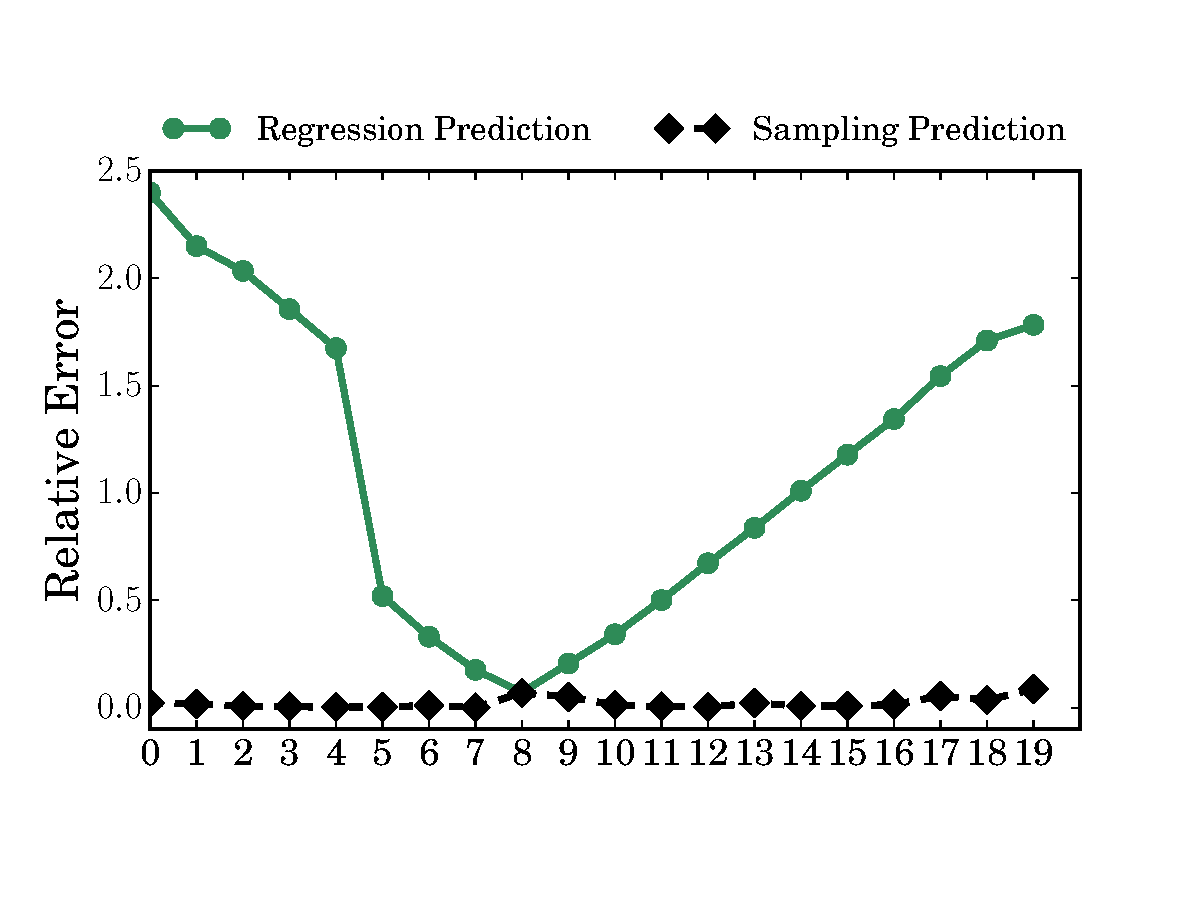
\includegraphics[width=0.6\textwidth]{../../PPoPP-2018/fig/prediction_relative_error.pdf}
	\bicaption[fig:prediction_relative_error]{Shuffle数据分布预测比较}{Shuffle数据分布预测比较}{Fig}{Prediction Relative Error of Range Partitioner}
\end{figure}

